\section{Benutzerf"uhrung}

\subsection{Elemente der grafischen Benutzeroberfl"ache}

\begin{figure}[htb]
\centering
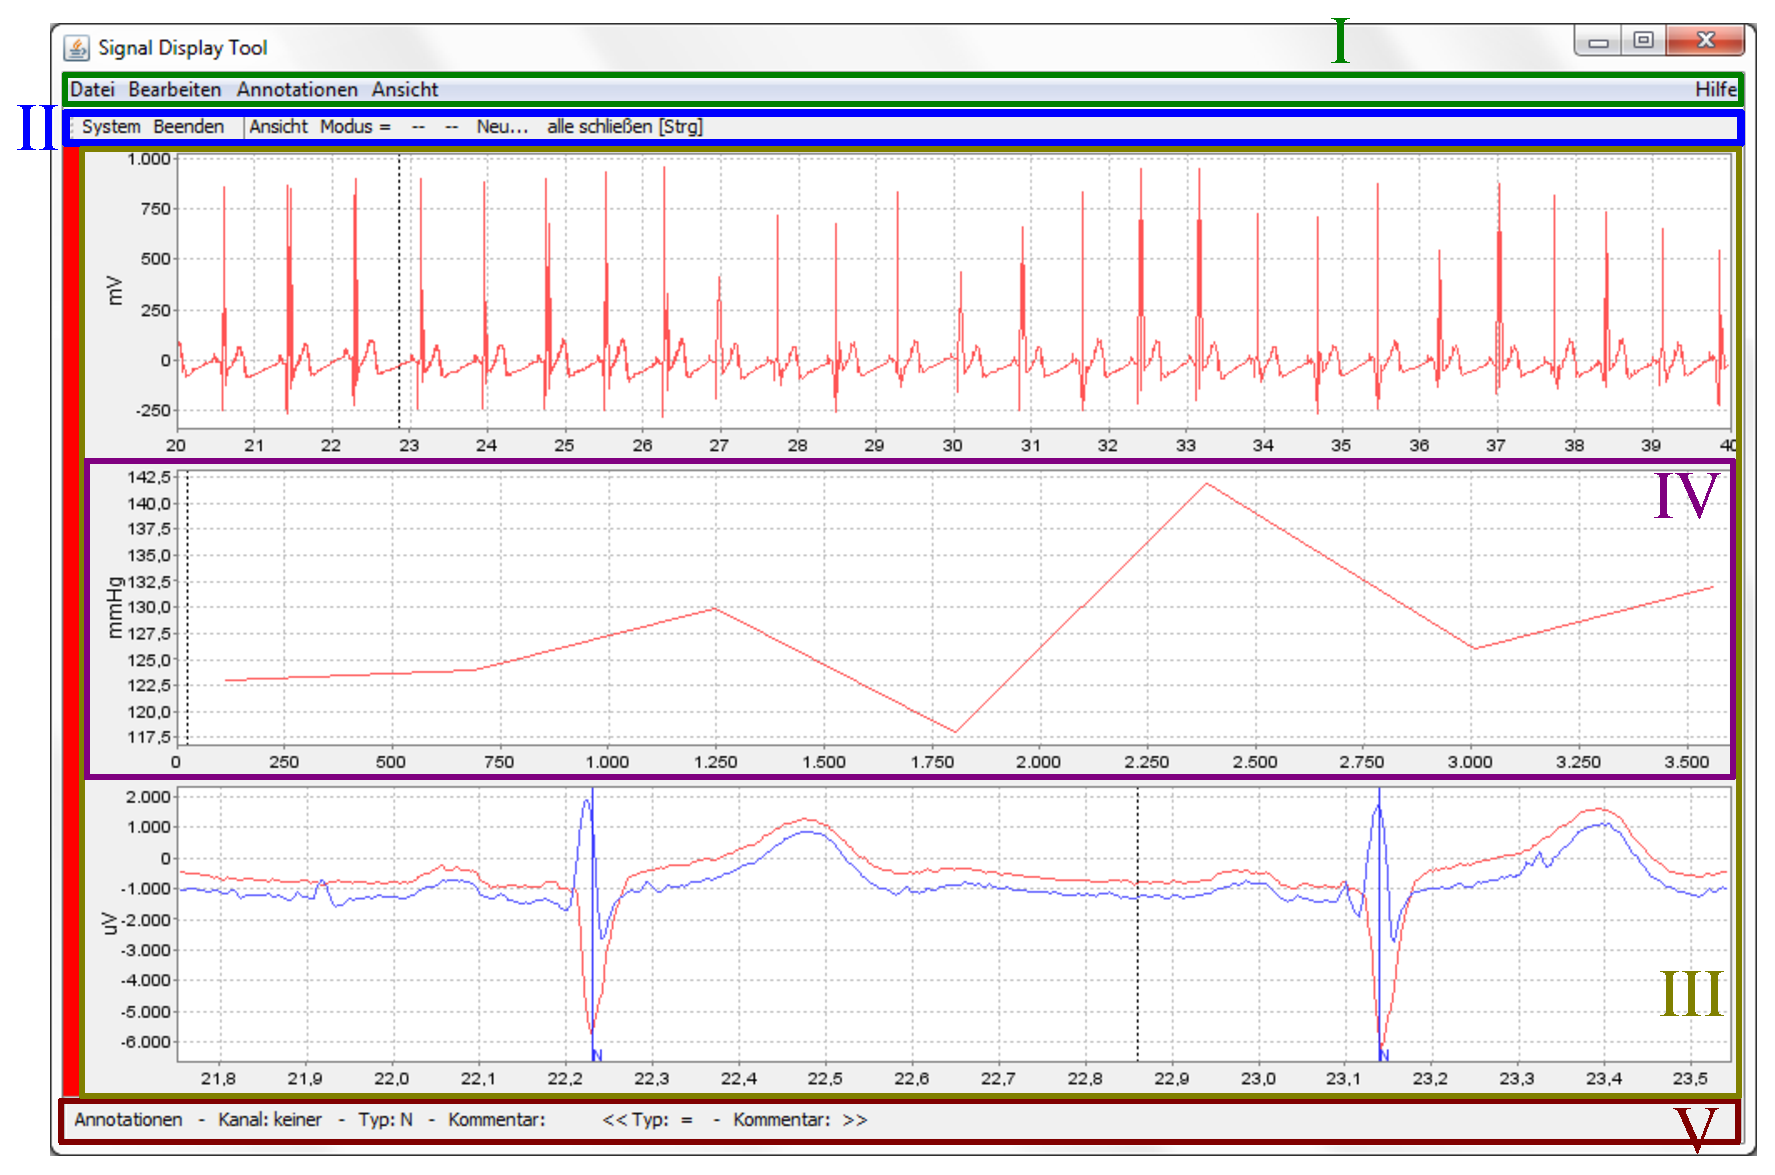
\includegraphics[width=\textwidth]{bilder/programm_ansicht.eps}
\caption[Klassen der grafischen Elemente]{Klassen der grafischen Elemente: I \texttt{Menus}, II \texttt{Toolbar}, III \texttt{SignalPanel}, IV \texttt{SignalView}, V \texttt{StatusBar}}
\label{pic:gui_elements_and_classes}
\end{figure}

In \picref{gui_elements_and_classes} sind die einzelnen Bestandteile der \ac{GUI} hervorgehoben.
Interaktionen zwischen dem Benutzer und dem Programm erfolgen "uber f"unf Hauptkomponenten:
\begin{itemize}
	\item Men"uzeile durch die Klasse \class{Menus} repr"asentiert
	\item Werkzeugleiste als Klasse \class{Toolbar}
	\item Statuszeile zum Anzeigen von Informationen mithilfe der Klasse \class{StatusBar}
	\item einzelne Diagramme als \class{SignalView}s zur Anzeige der Signalverl"aufe (im folgendem Signalansichten genannt)
	\item Zusammenfassung aller Signalansichten auf dem fl"achengr"o{\ss}tem Bestandteil, dem \class{SignalPanel}
\end{itemize}
W"ahrend das Men"u, die Werkzeugleiste und die Signalansichten Eingaben von dem Benutzer verarbeiten, dient die Statuszeile ausschlie{\ss}lich der Pr"asentation von Informationen.
Die grafische Darstellung der Klasse \class{SignalPanel} bleibt f"ur den Nutzer gr"o{\ss}tenteils verborgen, da es sich hierbei um ein organisatorisches Programmelement handelt (siehe dazu \secref{signalpanel_organisation}).

\begin{figure}[htb]
\centering
\includegraphics[angle=-90, width=0.9\textwidth]{bilder/package_ui_ubersicht.pdf}
\caption{"Ubersicht "uber das \class{ui}-Paket}
\label{pic:package_ui_ubersicht}
\end{figure}

Ein "Ubersicht die Klassenhierarchie ist in \picref{package_ui_ubersicht} dargestellt.
Bis auf die \class{SignalView}-Klasse sind alle grafischen Komponenten nach dem Singleton-Entwurfsmuster implementiert (vgl. \secref{singleton}).
Durch diese Entscheidung ist einerseits garantiert, dass die grafischen Elemente nur einmal in der Programminstanz vorkommen und au{\ss}erdem kann auf sie vereinfacht zugegriffen werden ("ahnlich globalen Variablen).

%- alle Elemente Singleton (bis auf \class{SignalView})

\subsection{Visualisierung der Signalverl"aufe}

\subsubsection{Die genutzte \jfcNS-Bibliothek}

F"ur die Darstellung der Signalverl"aufe in Diagrammen wird die \javaNS-Bibliothek \jfc genutzt.
\jfc wird, ebenso wie das \usNS-Format, unter der \ac{lgpl} zur freien Nutzung angeboten.
Mithilfe der \jfcNS-Bibliothek k"onnen Diagramm unterschiedlicher Art zur Visualisierung von Daten dargestellt werden.
Neben der Vielzahl der unterst"utzten Diagrammtypen werden zus"atzlich die dynamische ver"anderbare Graphen unterst"utzt.
%Zudem sind durch umfangreiche Einstellm"oglichkeiten die Diagramme ausgesprochen individualisierbar.
Die umfangreichen Einstellm"oglichkeiten bei der Anpassung der Diagramme erm"oglichen eine nahezu nahtlose Integration der Bibliothekselemente in das bestehende grafischen Gesamtbild.
Zudem bietet die \jfcNS-Bibliothek, zus"atzlich zur grafischen Veranschaulichung von Daten, auch grafische Elemente um Bereiche oder bestimmte Punkte in einem Diagramm gesondert hervorheben zu k"onnen.

%- Nutzung von \jfc (\ac{lgpl})
%- langsam bei der darstellung vieler Datenpunkte

\subsubsection{Die Wrapper-Klasse \class{SignalView}}

F"ur die Integration der Diagramme in die \ac{GUI} als Signalansichten existiert die Klasse \class{SignalView}.
Objekte der Klasse haben die Aufgabe, die durch die \class{DataController} bereit gestellten Daten dem Benutzer grafisch zu veranschaulichen.
\class{SignalView} ist eine Unterklasse der Klasse \class{ChartPanel} aus \jfc und bildet somit das Verbindungselement zwischen dem Programm und der genutzten Bibliothek.
Ein \class{SignalView}-Objekt ist somit grafisch ein Diagramm auf der Benutzeroberfl"ache (vgl. mit \picref{gui_elements_and_classes}).
Die Darstellung der Daten erfolgt durch zwei Varianten.
Darstellung von kontinuierlich abgetasteten Signalen (\emph{Signals}) und Einzelwertezeitreihen (\emph{Values}) erfolgt als Liniendiagramm der Werte "uber der Zeit.
Die grafische Pr"asentation von Annotationen ist durch senkrechte Striche in den Diagrammen realisiert.

Um die Daten darzustellen muss der entsprechende \class{DataController} der Signalansicht hinzugef"ugt werden.
Es wird sichergestellt, dass jeder \class{DataController} nur genau einmal ein und demselben \class{SignalView}-Objekt hinzugef"ugt werden kann.
Jeder \class{SignalView} kann beliebig viele \class{DataController}-Objekte speichern und darstellen.
\class{SignalView} implementiert das Interface \class{DataChangeListener} des \code{data}-Paketes und ist daher in der Lage dynamisch auf "Anderungen von Daten zu reagieren.
Wird z.\,B. eine Annotation durch den Benutzer dem Datensatz hinzugef"ugt oder ver"andert, so wird in jeder Signalansicht diese "Anderung auch grafisch dargestellt (sofern der entsprechende Kanal dargestellt wird).

Neben der grafischen Darstellung der Daten bietet die \class{SignalView}-Klasse weitere optische R"uckmeldung f"ur den Nutzer.
So wird die aktuelle Mausposition innerhalb eines Diagramms, in Bezug auf die Zeitachse (Abszisse) durch eine gestrichelte senkrechte Linie hervorgehoben.
Die Hervorhebung erfolgt nicht nur in dem Diagramm, "uber dem der Mauszeiger sich gerade befindet, sondern in allen dargestellten Diagrammen.
Zudem wird die Signalansicht, "uber der sich der Mauszeiger befindet, visuell durch Ver"anderung der Hintergrundfarbe markiert.
Damit ist f"ur den Nutzer ersichtlich, welches Diagramm seine Eingaben empf"angt.
Die Verarbeitung der Maus- und Tastatureingabe des Nutzers durch zwei innere Klassen \class{Signal\-View\-Mouse\-Adapter} und \class{Signal\-View\-Key\-Adapter}.
Details zur Behandlung der Benutzereingabe sind im \secref{userinput} weiter unten er"ortert.

Das genutzte \jfcNS-Paket bietet die M"oglichkeit einem Diagramm eine Datenreihe mit mehreren Tausend Datenpunkten zuzuordnen.
Die Wahl des darzustellenden Ausschnitts kann durch den Benutzer durchgef"uhrt werden und wird durch die Bibliothek komplett unterst"utzt.
Die Zeit, die die Bibliothek ben"otigt um ein Diagramm mit all seinen Komponenten darzustellen, sinkt mit der Anzahl der Datenpunkte.
Obwohl von \jfc ein Renderer (das Objekt dass die Datenpunkte in dem Diagramm darstellt) f"ur viele Datenpunkte angeboten wird, sinkt die Darstellungsgeschwindigkeit bei \unit{3000} oder mehr Datenpunkten so stark, dass die Aktualisierung der Anzeige nicht mehr fl"ussig erscheint.
Das Programm ben"otigt zu viel Zeit um die Diagramme auf dem Bildschirm zu zeichnen, dass die Verarbeitung der Benutzereingabe und die Darstellung merklich verz"ogert erfolgen.
Dieses Problem wird in der eingereichten Implementierung umgangen, indem den Diagramm-Objekten eine begrenzte Anzahl an Datenpunkten "ubergeben wird.
Die Zahl der dargestellten Datenpunkte ist auf die Breite in Pixeln der Diagramme festgelegt.
Damit bleibt die Darstellung fl"ussig aber es entstehen visuelle Artefakte die durch das Downsampling bedingt sind.
Diese Darstellungsartefakte nehmen mit Erh"ohung der Zoomstufe ab, da umso mehr Datenpunkte dargestellt werden, je kleiner der Signalausschnitt wird (gr"o{\ss}ere Pixelaufl"osung pro Zeiteinheit).

%- Klasse \class{SignalView}
%- erh"alt Daten von \class{DataController} aus dem \code{data}-Paket
%- unterscheidet nur zwischen Annotationen und Daten
%- Markierung der Mausposition durch \emph{Crosshair} (gestrichelte Linie)
%- Hervorhebung der Signalansicht, die gerade Mausfokus hat
%- Einschr"ankung durch Begrenzung der Punkte auf die Pixelbreite des entsprechenden Diagramms

\subsubsection{Dynamische Reaktion auf Ver"anderung der Daten}
\label{sec:dynamic_reaction}

Da durch die Implementierung in der Klasse \class{SignalView} die Darstellung der Daten von den Daten entkoppelt ist, resultiert eine "Anderung der Daten nicht direkt in einer "Anderung der Anzeige.
Es ist aber w"unschenswert diese Ver"anderungen dem Nutzer zu visualisieren.
Beispielsweise m"ochte der Benutzer eine neu hinzugef"ugte Annotation in allen Signalansichten dargestellt bekommen.
W"urde dies nicht geschehen, kann beim Nutzer Zweifel aufkommen, ob die Annotation erzeugt wurde oder nicht.
Um diese dynamische Aktualisierung der Anzeige zu erm"oglichen, wird durch die Klasse \class{SignalView} das Interface \class{DataChangeListener} implementiert (siehe \picref{package_ui_ubersicht}).
Sofern ein \class{DataController}-Objekt einer Signalansicht zugeordnet ist, wird das der Ansicht entsprechende \class{SignalView}-Objekt bei dem \class{DataController} als \class{DataChangeListener} registriert.
"Andern sich die Daten eines \class{DataController}s, wird diese Ver"anderung dem \class{SignalView}-Objekt mitgeteilt und es wird entsprechend das Diagramm aktualisiert.
Damit wird dem Nutzer eine visuelle R"uckmeldung bei "Anderungen der Daten geboten.

\subsection{Gr"o{\ss}enbestimmung und Positionierung der Signalansichten durch \class{SignalPanel}}
\label{sec:signalpanel_organisation}

Die Klasse \class{SignalPanel} "ubernimmt im \code{ui}-Paket eine organisatorische Rolle.
Sie umfasst innerhalb der \ac{GUI} den in \picref{gui_elements_and_classes} dargestellten Bereich III, wird aber durch die einzelnen Signalansichten verdeckt.
Eine Aufgabe von \class{SignalPanel} ist es, die einzelnen Signalansichten auf der zur Verf"ugung stehenden Fl"ache anzuordnen und deren Gr"o{\ss}en zu ver"andern.
Es werden drei Arbeitsmodi dem Benutzer zur Verf"ugung gestellt die "uber die Toolbar erreicht werden k"onnen:
\begin{itemize}
	\item gleiche Gr"o{\ss}en: Alle Signalansichten haben dieselbe H"ohe. Dieser Modus wird durch das = Symbol dargestellt.
	\item eine gro{\ss}e Ansicht: Eine Signalansicht wird auf \unit{60}{\%} der zur Verf"ugung stehende Gr"o{\ss}e dargestellt und alle restlichen sind verkleinert. Dieser Modus ist mit einer 1 gekennzeichnet.
	\item zwei vergr"o{\ss}erte Ansichten: Zwei Signalansichten erhalten jeweils \unit{35}{\%} der H"ohe zugesprochen und die restlichen sind verkleinert dargestellt. Diser Modus ist mit einer 2 gekennzeichnet.
\end{itemize}
Mit zwei zus"atzlichen Schaltfl"achen in der Toolbar k"onnen die zu vergr"o{\ss}ernden Signalansichten durch den Nutzer ausgew"ahlt werden.
Alle Signalansichten nutzten die komplette Breite und sind somit nur in ihrer H"ohe ver"anderlich.
Eine durch den Nutzer ver"anderliche Breite der Signalansichten ist nicht implementiert, da eine solche Funktionalit"at nicht notwendig ist und die Bedienung des Programms komplexer werden w"urde.
Neben der Positionierung und Anpassung der Gr"o{\ss}en "ubernimmt die \class{SignalPanel}-Klasse noch Koordinationsaufgaben bei dem gemeinsamen Scrollen und Zoomen der Signalansichten.
Diese Funktionen sind im folgendem Abschnitt beschrieben.

%- organisationseinheit

\subsection{Verarbeitung der Benutzereingabe im Paket \class{ui}}
\label{sec:userinput}

\subsubsection{Allgemeines zur Verarbeitung der Benutzereingaben}

Um auf Eingaben vom Benutzer reagieren zu k"onnen, besitzt die Klasse \class{SignalView} zwei innere Klassen: \class{Signal\-View\-Mouse\-Adapter} und \class{Signal\-View\-Key\-Adapter}.
Jedes \class{SignalView}-Objekt besitz jeweils eine Objektinstanz dieser beiden Klassen.
Die Methoden dieser Klassen werden durch aufgerufen, wenn ein Ereignis durch eine Maus- oder Tastatureingabe auftritt.
Diese Ereignisse werden durch \java immer an die grafische Komponente gesendet, die den Fokus der Anwendung h"alt.
In den meisten F"allen ist das die Komponente "uber der sich der Mauszeiger befindet.
Sobald die Maus in den Bildschirmbereich einer Signalansicht eintritt, wird diese durch eine Ver"anderung der Hintergrundfarbe hervorgehoben.
Gleichzeitig wird auch die Tastatureingabe an diese Signalansicht weitergeleitet.
Mit der optischen Hervorhebung der grafischen Komponente wird dem Nutzer eine R"uckmeldung dar"uber gegeben, welcher Teil des Programms (bzw. der Oberfl"ache) durch seine Eingaben ver"andert wird.
Beim Verlassen des Mauszeigers des grafischen Komponente wird die farbliche Hervorhebung wieder R"uckg"angig gemacht.

Beim Dr"ucken der L-Taste wird dem Nutzer eine Legende der dargestellten Signale eingeblendet, damit er die unterschiedlich farblichen Linien den Signalen zuordnen kann.
Dr"uckt der Benutzer die Taste E, so "offnet sich ein Dialog in dem er die Signale aus- und abw"ahlen kann die in der aktuellen Signalansicht dargestellt werden sollen.
Mit der Taste Q kann die Signalansicht geschlossen werden.
Zus"atzlich kann der Nutzer durch dr"ucken der Zifferntasten voreingestellte Annotationen ausw"ahlen, die er einem Annotationskanal hinzuf"ugen kann.
Der Vorgang der Editierung von Annotationen ist im \secref{edit_annotations} weiter unten beschrieben.
Die Behandlung der Eingaben des Nutzers zur Steuerung der Ansicht der einzelnen Signalansichten ist im folgendem Abschnitt beschrieben.

%- Einf"ugen und Entfernen von Datenkan"alen
%- Steuerung der Ansicht "uber Zeitfenster
%- Legende anzeigen
%- \class{SignalView} stellt dar
%- Datenzugriff "uber abstrakte Definition von \class{DataController}
%- Subklassen verarbeiten Maus- und Tastatureingabe

\subsubsection{Koordiniertes Zoomen und Scrollen "uber \class{SignalPanel}}

Die Darstellung der Signale erfolgt in Diagrammen.
Dabei wird die Abszisse als Zeitachse genutzt und die Werte der Zeitreihen werden auf der Ordinate abgebildet.
Der Wertebereich der Ordinate passt sich automatisch den dargestellten Signalen an.
Dabei wird die durch \jfc bereit gestellte Funktionalit"at das Minimum und das Maximum der Signalverl"aufe genutzt um den vertikalen vorhandenen Platz optimal zu nutzen.
Der Wertebereich der Abszissenachse kann durch den Nutzer mithilfe der Maus ver"andert werden.
Durch drehen des Mausrades wird der Wertebereich verschoben und der Nutzer scrollt entlang der Zeitachse die Signalansicht.
Wird die Gro{\ss}schreibtaste w"ahrend der Mausradbewegung gedr"uckt, wird der Wertebereich vergr"o{\ss}ert bzw. verkleinert - der Anwender zoomt in einen Zeitbereich hinein oder hinaus.
Der Wert um wieviel Zeiteinheiten gezoomt bzw. gescrollt wird ist proportional zu der Gr"o{\ss}e des dargestellten Zeitbereichs und betr"agt \unit{15}{\%} des dargestellten Zeitabschnitts.
Der zentrale Wert des dargestellten Zeitbereichs bleibt w"ahrend des Zoomens unver"andert.
Wird mit der mittleren Maustaste innerhalb einer Signalansicht geklickt, so wird die Ansicht auf den angeklickten Zeitpunkt zentriert.
Die Zoomstufe und somit die Breite des Zeitbereichs bleibt dabei konstant.

Da die einzelnen Diagramme und ihre Daten "ublicherweise in ihrem Zusammenhang betrachtet werden, ist es notwendig die Ver"anderungen der Ansicht in einem Diagramm an die anderen Diagramme zu "ubergeben.
Es soll ein Effekt erreicht werden, dass alle Signale (egal in welchem Diagramm dargestellt) "uber ein und derselben Zeitachse dargestellt werden.
Hierf"ur ruft die Klasse \class{Signal\-View\-Mouse\-Adapter} nicht die Methoden des ihnen zugeordneten \class{SignalView}-Objektes auf, sondern gibt die Informationen "uber den darzustellenden Zeitbereich an die Klasse \class{SignalPanel} weiter.
Erst in den Methoden \code{ScrollToActionEvent()} und \code{ZoomActionEvent()} der Klasse \class{SignalPanel} werden anschlie{\ss}end die Methoden der \class{SignalView}-Objekte aufgerufen.
Es wird in den Methoden von \class{SignalPanel} gepr"uft ob ein koordiniertes Zoomen bzw. Scrollen f"ur den urspr"unglichen \class{SignalView} aktiviert ist.
Ist die koordinierte Ansichtssteuerung aktiv, werden alle Ansichten auf den gew"ahlten Zeitbereich gestellt.
Nur wenn die Koordination deaktiviert ist, wird nur der Zeitbereich des \class{SignalView}s ver"andert bei dem die Nutzereingabe aufgetreten ist.
Es k"onnen das koordinierte Zoomen und Scrollen unabh"angig voneinander f"ur alle Signalansichten aktiviert bzw. deaktiviert werden.

%- Observer-Prinzip
%- zwei eigene Managerklassen (Unabh"angigkeit) \class{ScrollLockManager}, \class{ZoomLockManager}

\subsubsection{Verarbeitung und Ver"anderung von Annotationen}
\label{sec:edit_annotations}

Annotationen k"onnen durch den Benutzer erstellt, editiert und gel"oscht werden.
Sie werden nicht wie \emph{Values} und \emph{Signals} als Liniendiagramm dargestellt, da sie keinen Zahlenwert an sich besitzen.
F"ur sie wird eine senkrechte Linie an dem entsprechenden Zeitpunkt gezeichnet.
Zum Ver"andern der Annotationen wird auf die Klasse \class{AnnotationManager} des \code{data}-Paketes zur"uck gegriffen.
Diese Klasse ben"otigt einen Eintrag eines Datensatzes damit bekannt ist, wo die Annotationen im Datensatz abgespeichert werden sollen.
Der Nutzer kann "uber das Men"u den Datensatzeintrag ausw"ahlen und der entsprechende \class{DataController} wird an den \class{AnnotationManager} "ubergeben.

Klickt der Benutzer in einem \class{SignalView} wird eine neue Annotation erzeugt und in dem ausgew"ahltem Datensatzeintrag abgespeichert.
Dr"uckt der Nutzer bei dem Mausklick die Gro{\ss}schreibtaste kann er mithilfe eines Dialogfensters das Symbol und den Kommentar zu dieser Annotation editieren.
Er kann auch aus vier implementierten Voreinstellungen f"ur Symbol und Kommentar per Druck auf eine Zifferntaste ausw"ahlen.
Erfolgt der Mausklick ohne weitere zus"atzliche Tastendr"ucke wird die Annotation mit den zuletzt genutzten Symbol und Kommentar erzeugt.
Durch diese Handhabe wird dem Nutzer die Eingabe mehrerer gleichartiger Annotationen erleichtert.
Die Information zu dem Symbol und dem Kommentar werden durch den \class{AnnotationManager} zwischengespeichert.

Die Bestimmung der Zeitpunkte an denen die Annotationen eingef"ugt werden sollen, erfolgt durch die Klasse \class{Signal\-View\-Mouse\-Adapter}.
Dabei wird der Zeitpunkt aus der relativen X-Koordinate des Mausklicks zu der Abszisse errechnet.
Der errechnete Zeitpunkt muss zus"atzlich noch auf den n"achstgelegenen Zeitpunkt der mit der virtuellen Abtastrate "ubereinstimmt gerundet werden.
Erfolgt der Klick au{\ss}erhalb des durch die Koordinatenachsen aufgespannten Bereichs wird keine Annotation eingef"ugt.
Zum L"oschen von Annotationen muss durch den Nutzer beim Klick die Steuerungstaste gedr"uckt werden.
Erfolgt der Druck der Maustaste auf dem der Annotation angeheftetem Symbol, kann die selektierte Annotation durch den Anwender verschoben werden.
Den Zustand, dass der Anwender eine Annotation durch den Nutzer gerade verschoben wird, ist durch eine farbliche Ver"anderung des Mauszeigers dargestellt.

Da die senkrechten Linien zur Repr"asentation der Annotationen durch die \jfcNS-Bibliothek nicht als eigene grafische Objekte zur Verf"ugung gestellt werden, k"onnen auch die Zeitpunkte der repr"asentierten Annotationen nicht direkt erhalten werden.
Im Programm erfolgt die Zeitbestimmung des der Position des Mausklicks innerhalb des Diagramms wie beim Einf"ugen von Annotationen und mithilfe dieses Zeitpunktes wird die entsprechende Annotation im selektierte Annotationskanal gesucht.
Intern wird hier in einem kleinen Zeitbereich gesucht, da der Nutzer pixelgenau klicken m"usste, wenn nur der spezielle Zeitpunkt ausgew"ahlt werden w"urde.
Der Zeitbereich ist in diesem Fall auch wieder relativ zur dargestellten Bereich gew"ahlt und betr"agt \unit{1}{\%} dessen.
Mithilfe dieser Implementierung wird dem Nutzer erm"oglicht auch mit "`ungenauen"' Mausklicks genau die Annotationen zu selektieren die er ver"andern m"ochte.
Das vereinfacht die Bedienung erheblich.
Durch die im \secref{dynamic_reaction} beschriebene Implementierung des \class{DataChangeListener}-Interfaces wird beim Ver"andern einer Annotation alle Ansichten, die diese Annotation darstellen, automatisch aktualisiert.
Der Nutzer erh"alt sofort eine optische R"uckmeldung "uber die von ihm vorgenommenen "Anderungen.

%- Einf"ugen von Annotationen "uber \class{AnnotationManager}
%- Dreiecksbeziehung von \class{Annotation\-Controller}, \class{AnnotationList} und \class{AnnotationManager} erl"autern
%- Suchalgorithmus zum finden der aktuellen Annotation
%- "Anderung wird durch die Implementierung vom Interface \class{Data\-Change\-Listener} automatisiert aktualisiert

% EOF
